% 常见几何体的转动惯量

\pentry{转动惯量\upref{RigRot}}

\begin{figure}[ht]
\centering
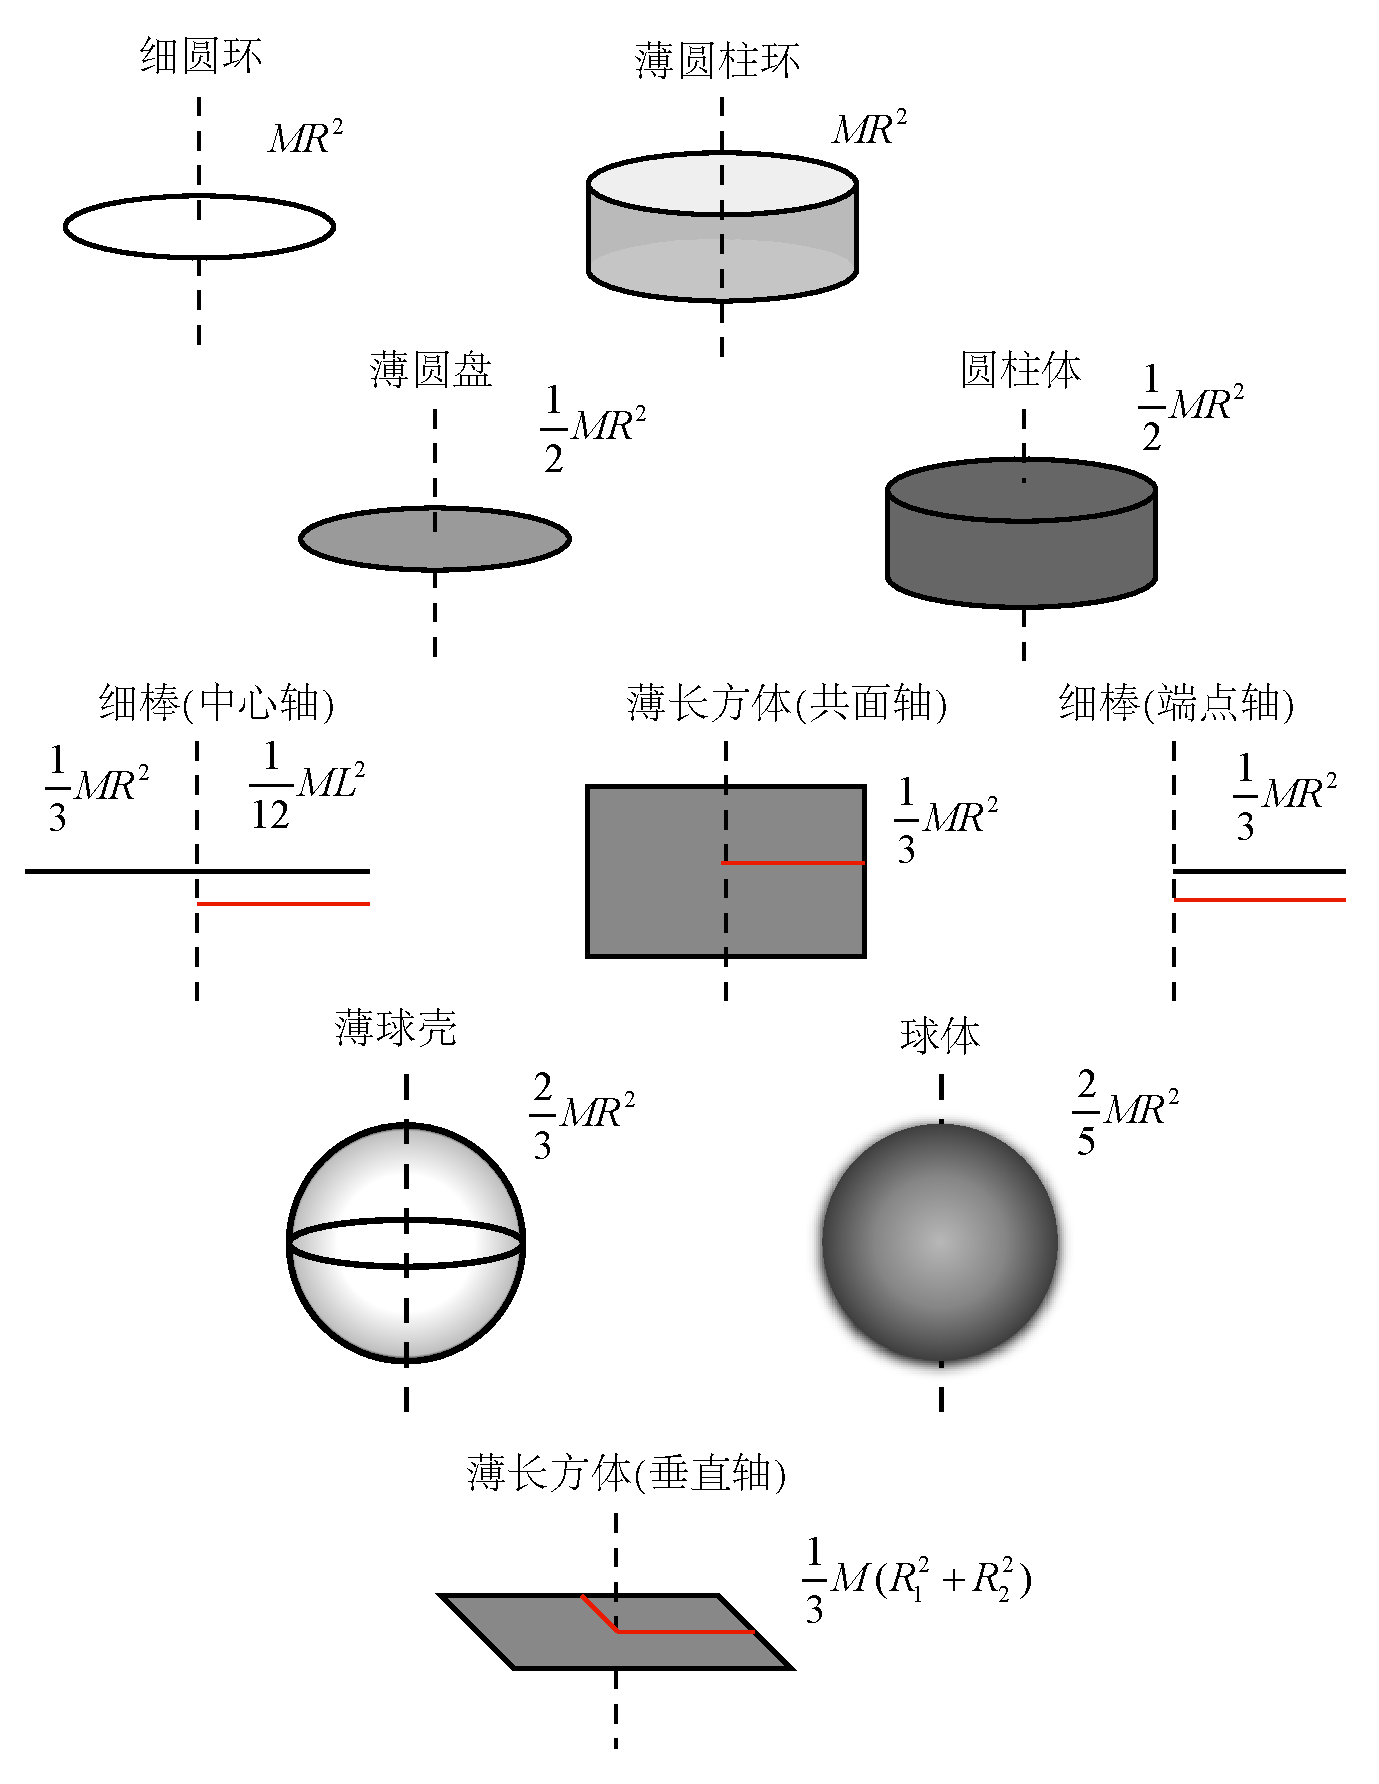
\includegraphics[width=12cm]{./figures/ExMI.pdf}
\caption{常见几何体的转动惯量,虚线为转轴,物体质量 $M$ 均匀分布, $R$ 为几何体的半径或红线标注的长度.}\label{ExMI_fig1}
\end{figure}

\subsection{细圆环\ 薄圆柱环}
细圆环和薄圆柱环的所有质量与转轴的距离都为 $R$,可以看成许多质点的叠加,每个质点转惯量为 $m_i R^2$,所以
\begin{equation}
I = \sum\limits_i {{m_i}{R^2}}  = M{R^2}
\end{equation}

\subsection{ 细棒(端点轴)}
细棒的线密度为 $\lambda  = M/L$,如果划分成长度为 $\D r$ 的小段,第 $i$ 段距离转轴 $r_i$

\subsection{细棒(中心轴)\ 薄长方体(共面轴)}
细棒(中心轴)可以看做两个等质量的细棒(端点轴),质量分都为 $M_1$,每个具有转动惯量 $M_1 R^2/3$, 总转动惯量为 $2M_1 R^2/3=MR^2/3$.由此可以看出,\textbf{若一个物体可以拆分成转动惯量相同的若干部分,那么转动惯量公式不变}.薄长方体(共面轴)可以看成许多许多细棒(中心轴)组成,所以转动惯量的系数仍然为 $1/3$. 注意一些教材中使用细棒的总长度 $L=2R$, 则转动惯量为 $ML^2/12$.

\subsection{薄圆盘\ 圆柱}
薄圆盘可以看做许多宽度为 $\D r$ 的细圆环组成\footnote{然而不能看做由许多过圆心的细棒组成,因为这样面密度就是不均匀的.另外注意每个细环的转动惯量并不相同(因为半径各不相同),所以不能直接用圆环的转动惯量公式.},质量面密度为 $\sigma  = M/\pi {R^2}$,第 $i$ 个圆环的半径为 $r_i$,面积为 $2\pi r_i\D r$,总转动惯量为
\begin{equation}
I = \sum\limits_i {r_i^2\D{m_i}}  = \sum\limits_i {r_i^2 \vdot \sigma  \vdot 2\pi {r_i}\D r}  = 2\pi \sigma \sum\limits_i {r_i^3\D r}  = 2\pi \sigma \int_0^R {{r^3}\D r}
\end{equation}
也可以在极坐标中直接根据定义写出积分
\begin{equation}
I = \int {{r^2}\sigma \D s}  = \int_0^{2\pi } {\int_0^R {\sigma {r^2} \vdot r\D r\D\theta } }  = 2\pi \sigma \int_0^R {{r^3}\D r}  = \frac{1}{2}\sigma \pi {R^2}{R^2} = \frac{1}{2}M{R^2}
\end{equation}
圆柱可看做许多相同的薄圆盘组成,转动惯量系数相同.

\subsection{薄球壳}
球壳可以看做许多细圆环组成,质量面密度为 $\sigma  = M/4\pi {R^2}$,球坐标中,令第 $i$ 个圆环对应的极角为 $\theta$,宽度为 $R\D \theta$,面积为 $\D{s_i} = 2\pi R\sin {\theta _i} \vdot R\D\theta$,半径为 ${r_i} = R\sin {\theta _i}$,总转动惯量为
\begin{equation}\label{ExMI_star}
\begin{gathered}
  I = \sum\limits_i {r_i^2\D{m_i}}  = \sum\limits_i {{R^2}{{\sin }^2}{\theta _i} \vdot \sigma  \vdot 2\pi R\sin {\theta _i} \vdot R\D\theta }  \hfill \\
   = 2\pi \sigma {R^4}\sum\limits_i {{{\sin }^3}{\theta _i}\D\theta }  = 2\pi \sigma {R^4}\int_0^\pi  {{{\sin }^3}\theta \D\theta }  \hfill \\ 
\end{gathered}
\end{equation}
也可以在球坐标中直接写出球面积分
\begin{equation}
\begin{gathered}
  I = \int {{r^2}\sigma \D s}  = \int_0^{2\pi } {\int_0^\pi  {{{(R\sin \theta )}^2} \vdot \sigma  \vdot {R^2}\sin \theta \D\theta \D\phi } }  = 2\pi \sigma {R^4}\int_0^\pi  {{{\sin }^3}\theta \D\theta }  \hfill \\
   = 2\pi \sigma {R^4}\int_{ - 1}^1 {(1 - {{\cos }^2}\theta )\D\cos \theta }  = \frac{2}{3}(\sigma 4\pi {R^2}){R^2} = \frac{2}{3}M{R^2} \hfill \\ 
\end{gathered}
\end{equation}
其中对 $\theta$ 的积分使用了换元积分法.%(链接未完成,最好有链接到例题) 

\subsection{球体}
球体可以看做许多薄球壳组成,体密度为 $\rho  = M/(4\pi {R^3}/3)$,令第 $i$ 个球壳半径为 $r_i$,厚度为 $\D r$,体积为 $4\pi r_i^2\D r$,总转动惯量为
\begin{equation}
I = \sum\limits_i {\frac{2}{3}{m_i}r_i^2}  = \frac{2}{3}\sum\limits_i {\rho {V_i}r_i^2}  = \frac{2M}{R^3}\sum\limits_i {r_i^4\D r}  = \frac{2M}{R^3}\int_0^{ + \infty } {{r^4}\D r}
\end{equation}
也可以在球坐标中直接体积分
\begin{equation}
\begin{aligned}
I &= \int {{{(r\sin \theta )}^2}\D m}  = \int_0^{2\pi } {\int_0^\pi  {\int_0^R {{{(r\sin \theta )}^2}\sigma {r^2}\sin \theta \D r\D\theta \D\phi } } } \\
&= \frac{3M}{2R^3}\int_0^\pi  {{{\sin }^3}\theta \D\theta } \int_0^R {{r^4}\D r}  =\frac{2M}{R^3}\int_0^R {{r^4}\D r}  = \frac{2}{5}M{R^2}
\end{aligned}
\end{equation}
其中对 $\theta$ 的积分使用了换元积分法.%(链接未完成,最好有链接到例题)

\subsection{薄长方体(垂直轴)}
由“薄长方体(共面轴)”可知两个共面方向的转动惯量分别为 $MR_1^2/3$ 和 $MR_2^2/3$,使用平行轴定理%(未完成)
可得关于垂直轴的转动惯量为二者之和
\begin{equation}
I = \frac{1}{3} (MR_1^2+MR_2^2)
\end{equation}